\documentclass[12pt]{article}
\usepackage{graphicx}

\usepackage{xcolor}
\usepackage{hyperref}
\usepackage{float}
\usepackage{amsmath}
\usepackage{etoolbox}
\usepackage{tikz}
\usetikzlibrary{calc,patterns,angles,quotes}
\usepackage{gensymb}

\usepackage[T1]{fontenc} 							% imposta la codifica dei font
\usepackage[utf8]{inputenc} 							% lettere accentate da tastiera
\usepackage[english]{babel} 							% per scrivere in italiano
\addto{\captionsenglish}{\renewcommand{\bibname}{List of References}}


\usepackage{footmisc}


\usepackage{fancyhdr}
\usepackage{longtable}


\usepackage{subfig}


\usepackage{listings}


\definecolor{mGreen}{rgb}{0,0.6,0}
\definecolor{mGray}{rgb}{0.5,0.5,0.5}
\definecolor{mPurple}{rgb}{0.58,0,0.82}
\definecolor{backgroundColour}{rgb}{0.95,0.95,0.92}

\lstdefinestyle{CStyle}{
    backgroundcolor=\color{backgroundColour},   
    commentstyle=\color{mGreen},
    keywordstyle=\color{magenta},
    numberstyle=\tiny\color{mGray},
    stringstyle=\color{mPurple},
    basicstyle=\footnotesize,
    breakatwhitespace=false,         
    breaklines=true,                 
    captionpos=b,                    
    keepspaces=true,                 
    numbers=left,                    
    numbersep=5pt,                  
    showspaces=false,                
    showstringspaces=false,
    showtabs=false,                  
    tabsize=2,
    language=C
}

\addtolength{\headheight}{1.5cm} % make more space for the header
\pagestyle{fancyplain} % use fancy for all pages except chapter start
\lhead{\includegraphics[height=0.1cm]{./Images/logo_hidden.png}} % left logo
\rhead{\includegraphics[height=2.3cm]{./Images/logo.png}} % right logo
\renewcommand{\headrulewidth}{0pt} % remove rule below header

\usepackage[colorinlistoftodos]{todonotes}

\newcommand\tab[1][1cm]{\hspace*{#1}}

\newcommand{\nrange}[4][]{%
  #2=%
  \ifblank{#1}{% Optional argument empty? Yes? Then omit the second number in the enumeration
    #3, \dots ,#4%
  }{%
    #3, #1, \dots,#4%
  }%
}

\begin{document}

\begin{titlepage}

\newcommand{\HRule}{\rule{\linewidth}{0.5mm}} % Defines a new command for the horizontal lines, change thickness here

\center % Center everything on the page
 
%----------------------------------------------------------------------------------------
%	HEADING SECTIONS
%----------------------------------------------------------------------------------------

\textsc{\LARGE La Sapienza University}\\[1.5cm] % Name of your university/college
\textsc{\Large Department of Computer Science}\\[0.5cm] % Major heading such as course name
\textsc{\large Autonomous Networking}\\[0.5cm] % Minor heading such as course title

%----------------------------------------------------------------------------------------
%	TITLE SECTION
%----------------------------------------------------------------------------------------

\HRule \\[0.4cm]
{ \huge \bfseries Report HomeWork 3}\\[0.4cm] % Title of your document
\HRule \\[1.5cm]
 
%----------------------------------------------------------------------------------------
%	AUTHOR SECTION
%----------------------------------------------------------------------------------------

\begin{minipage}{0.4\textwidth}
\begin{flushleft} \large
\emph{Authors:}\\
Giordano \textsc{Dionisi} 1834919 \\
Mattia \textsc{Lisi} 1709782 \\
Michele \textsc{Spina} 1711821 \\

\end{flushleft}
\end{minipage}
~
\begin{minipage}{0.4\textwidth}
\begin{flushright} \large
\emph{Supervisor:} \\
Prof. Andrea \textsc{Coletta} % Supervisor's Name

\emph{Co-Supervisor:} \\
Prof.ssa Gaia \textsc{Maselli} % Supervisor's Name

\end{flushright}
\end{minipage}\\[2cm]

% If you don't want a supervisor, uncomment the two lines below and remove the section above
%\Large \emph{Author:}\\
%John \textsc{Smith}\\[3cm] % Your name

%----------------------------------------------------------------------------------------
%	DATE SECTION
%----------------------------------------------------------------------------------------

{\large \today}\\[2cm] % Date, change the \today to a set date if you want to be precise

%----------------------------------------------------------------------------------------
%	LOGO SECTION
%----------------------------------------------------------------------------------------

\includegraphics[height=3.8cm]{./Images/logo_firstpage.png}\\[3cm] % Include a department/university logo - this will require the graphicx package
 
%----------------------------------------------------------------------------------------

\vfill % Fill the rest of the page with whitespace


\end{titlepage}

\tableofcontents

\newpage

\section{Formalize The Problem}

We have this scenario:

\begin{itemize}

    \item Two Depots:
  
    \[
        \nu = Depot -1  
    \]
    \[
        \pi = Depot -2
    \]
    
    \item $\eta$ drones
    
    \item Each drone $\theta$ has $\Gamma(\theta)$ packets
    
\end{itemize}

We want build a routing algorithm to allow drones to communicate each other for the purpose to get arrive as much as possible $\Gamma$ to the $\nu$ and $\pi$.
\\
\\
Graphically the Scenario is:

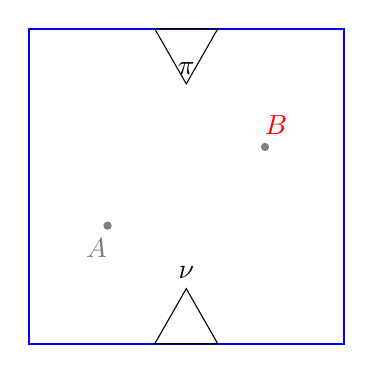
\begin{tikzpicture}
    %\draw[step=1cm,gray,very thin] (-2,-2) grid (2,2);
    \draw[blue, thick] (-2,-2) rectangle (2,2);
    
    
    \draw (0.4, -2) node[anchor=north]{}
  -- (-0.4,-2) node[anchor=north]{}
  -- (0,-1.3) node[anchor=south]{$\nu$}
  -- cycle;
  \draw (0.4, 2) node[anchor=north]{}
  -- (-0.4, 2) node[anchor=north]{}
  -- (0,1.3) node[anchor=south]{$\pi$}
  -- cycle;
  
  \fill [color=gray] (-1,-0.5) circle (1.5pt);
  \draw[color=gray] (-1.14,-0.78) node {$A$};
  
  \fill [color=gray] (+1,+0.5) circle (1.5pt);
  \draw[color=red] (+1.14,+0.78) node {$B$};
  
\end{tikzpicture}

\textbf{Where:}

$A$ and $B$ are two \textit{drones.}

\section{Solution}

First of all we divide the scenario in \textit{grids:}

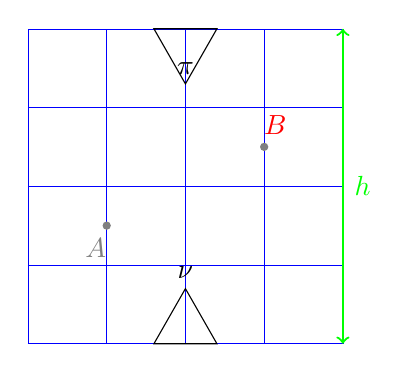
\begin{tikzpicture}
    \draw[step=1cm,blue,very thin] (-2,-2) grid (2,2);
    \draw (0.4, -2) node[anchor=north]{}
  -- (-0.4,-2) node[anchor=north]{}
  -- (0,-1.3) node[anchor=south]{$\nu$}
  -- cycle;
  \draw (0.4, 2) node[anchor=north]{}
  -- (-0.4, 2) node[anchor=north]{}
  -- (0,1.3) node[anchor=south]{$\pi$}
  -- cycle;
  
  \fill [color=gray] (-1,-0.5) circle (1.5pt);
  \draw[color=gray] (-1.14,-0.78) node {$A$};
  
  \fill [color=gray] (+1,+0.5) circle (1.5pt);
  \draw[color=red] (+1.14,+0.78) node {$B$};
  
  \draw[thick,<->, green] (2,-2) -- (2,2);
  
  \draw[color=green] (2.25,0) node {$h$};
  
\end{tikzpicture}

\textbf{Where:} 

\begin{itemize}

\item {\color{green}{$h$}} $\Rightarrow$ Lenght of one side of the square of grid.

\end{itemize}

After we need to define States\ref{subsection:States}, Actions\ref{subsection:Actions} and Reward\ref{subsubsection:Reward}

\subsection{States}
\label{subsection:States}

Each cell $\chi$ of the grid built is a state for the system. So each $\theta$ isn't a state, but it takes the state of the particular $\chi$ where it stays.

Formally we have:

\[
\omega = 4
\]
\[
\Lambda = 4
\]

\textbf{Where:}

\begin{itemize}

    \item $\omega$: Number of cells on \textit{X axis}

    \item $\Lambda$: Number of cells on \textit{Y axis}

\end{itemize}
$\Omega$ is the total amount of cells in the grid:

\[
\Omega = \omega * \Lambda
\]

Let's define:

\begin{itemize}

    \item Each $\chi$ is defined by a left bottom point $X$ and a right upper point $Y$, so each $\chi$ is defined by a bounding-box.
    
\end{itemize}

    
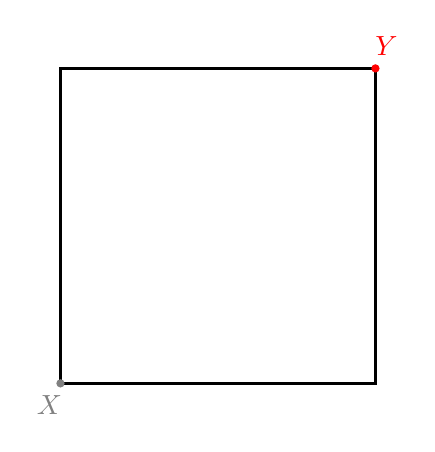
\begin{tikzpicture}
    %\draw[step=1cm,gray,very thin] (-2,-2) grid (2,2);
    \draw[black, very thick] (-2,-2) rectangle (2,2);
    
    \fill [color=gray] (-2,-2) circle (1.5pt);
    \draw[color=gray] (-2.14,-2.28) node {$X$};
        
    \fill [color=red] (+2,+2) circle (1.5pt);
    \draw[color=red] (+2.14,+2.28) node {$Y$};

\end{tikzpicture}

    
Each $X$ and $Y$ for each $\chi$ are defined by:


\begin{lstlisting}[style=CStyle, texcl=<true|false>, mathescape=true]
for i=0 to $h$:

    for j=0 to $h$:
    
        $\chi$[$X$] = [i; j]
        $\chi$[$Y$] = [i + ($\frac{h}{\omega}$); j + ($\frac{h}{\omega}$)]
        j = j + $\frac{h}{\omega}$
        
    i = i + $\frac{h}{\omega}$
\end{lstlisting}
    
\textbf{Where:}

\begin{itemize}

    \item $\chi[X]$ $\Rightarrow$ coordinate X of $\chi$

    \item $\chi[Y]$ $\Rightarrow$ coordinate Y of $\chi$

\end{itemize}

Each State of System $\equiv$ Each $\chi$ \\

\textit{\textbf{Brief Recap}}

We divide the area (h,h) of grid with a regular tessellation\footnote{$\Omega$ cells.}. Each $\chi$ of the grid delimits an internal space in the grid that we will use as one state for the $\theta$.

When a $\theta$ stays in a particular $\chi$, it takes its particular state.

\subsection{Actions}
\label{subsection:Actions}



\begin{minipage}{0.45\textwidth}
The following: \\

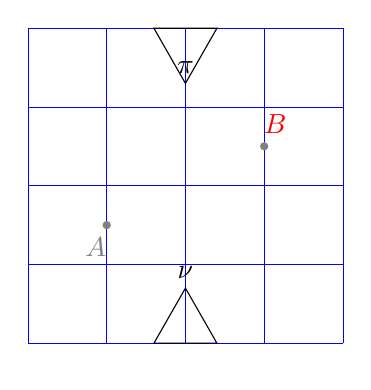
\begin{tikzpicture}
    \draw[step=1cm,blue,very thin] (-2,-2) grid (2,2);
    \draw (0.4, -2) node[anchor=north]{}
  -- (-0.4,-2) node[anchor=north]{}
  -- (0,-1.3) node[anchor=south]{$\nu$}
  -- cycle;
  \draw (0.4, 2) node[anchor=north]{}
  -- (-0.4, 2) node[anchor=north]{}
  -- (0,1.3) node[anchor=south]{$\pi$}
  -- cycle;
  
  \fill [color=gray] (-1,-0.5) circle (1.5pt);
  \draw[color=gray] (-1.14,-0.78) node {$A$};
  
  \fill [color=gray] (+1,+0.5) circle (1.5pt);
  \draw[color=red] (+1.14,+0.78) node {$B$};
  
\end{tikzpicture}
\end{minipage}%
\hfill
\begin{minipage}{0.45\textwidth}
Becomes this: \\

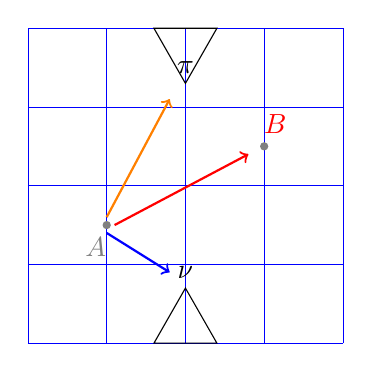
\begin{tikzpicture}
    \draw[step=1cm,blue,very thin] (-2,-2) grid (2,2);
    \draw (0.4, -2) node[anchor=north]{}
  -- (-0.4,-2) node[anchor=north]{}
  -- (0,-1.3) node[anchor=south]{$\nu$}
  -- cycle;
  \draw (0.4, 2) node[anchor=north]{}
  -- (-0.4, 2) node[anchor=north]{}
  -- (0,1.3) node[anchor=south]{$\pi$}
  -- cycle;
  
  \fill [color=gray] (-1,-0.5) circle (1.5pt);
  \draw[color=gray] (-1.14,-0.78) node {$A$};
  

  \draw[thick,->, orange] (-1,-0.4) -- (-0.2,1.1);
  \draw[thick,->, blue] (-1,-0.6) -- (-0.2,-1.1);
  
  \fill [color=gray] (+1,+0.5) circle (1.5pt);
  \draw[color=red] (+1.14,+0.78) node {$B$};
  \draw[thick,->, red] (-0.9,-0.5) -- (0.8,0.4);
  
\end{tikzpicture}
\end{minipage}%
\hfill

Let's assume we are $A$\footnote{This does not make you lose generality.}

Let's define:

\begin{itemize}

    \item $N(A)$ is the set of neighbors for $A$\footnote{Nodes in its communication range.}.
    
\end{itemize}
    
In each moment if $A$ has a packet $\psi$, then $A$ can perform different actions:


\begin{itemize}

    \item $A$ can mantain $\psi$;

    \item $A$ can go to $\nu$;

    \item $A$ can go to $\pi$;

    \item $A$ can pass $\psi$ to a $B$ $\in$ $N(A)$.
    
\end{itemize}
    
The particular action $\beta$ chosen depends on:

\[
    \beta= 
    \begin{cases}
        \text{Q-Learning},& \text{if } \ni\leq 1-\epsilon\\
        \text{Modified MGEO},& \text{otherwise}
    \end{cases}
\]

Where $\ni$ is a random value\footnote{This is explained in \ref{subsection:Continue_Actions}.}. \\

We based our algorithm on \textit{Epsilon-Greedy Approach.} \\

First of all let's define $\epsilon$.

\subsubsection{Epsilon}

$\epsilon$ is defined by the following function:

\[
    \epsilon[\theta] = \frac{1}{\kappa}
\]

\begin{itemize}

    \item $\epsilon$ is computed locally for each $\theta$.

    \item $\kappa$ is variable that represents the number of times that $\theta$ has updated its Q-Sets.

    \[
        \kappa = 1, 2, 3,\dots,+\infty
    \]

    \begin{figure}[H]

        \includegraphics[width=\textwidth,height=\textheight,keepaspectratio]{./Images/1_x.png}
                
        \caption{Plot $\frac{1}{\kappa}$}
                
    \label{fig:figure1}
    \end{figure}

\end{itemize}
As can be seen in Figure \ref{fig:figure1}, $\epsilon$ function, defined in [1, $+\infty$], is a continuous decreasing function with initial value $S = 1$ and it tends to zero for high value of $\kappa$.

In this way the probability of using \textit{Q-learning} approach will be directly proportional to the amount of information received ($\kappa$), so using it more when it's more effective. At the same time when the algorithm haven't some information, then the use of \textit{Modified MGEO} approach is almost a certain event.

\textit{\textbf{Just for Completeness}}

Algorithm is based on \textbf{Optimistic Initial Value $\mu$.} Sperimentally best value is:

\[
    \mu = 10 
\]

Indeed \textit{\textbf{initially}} it's privileged \textit{higher \textbf{exploration} than \textbf{exploitation,}} so $\mu$ must be enough higher than upper value of Reward\ref{subsubsection:Reward}.

\subsubsection{Reward}
\label{subsubsection:Reward}

The Reward $\lambda$ is related to the delayed outcome $\iota$ of the specific packet $\psi$:

\[
    \lambda= 
    \begin{cases}
        -1,& \text{if } \iota = -1\\
        1 + \frac{\sigma - \xi}{\sigma}, & \text{otherwise}
    \end{cases}
\]

\textbf{Where:}

\begin{itemize}

    \item $\sigma$: \textit{Time-To-Live} for $\psi$

    \item $\xi$: Delay of $\psi$, so:
    
    \[
        \xi \in [0, \sigma]
    \]
    
\end{itemize}

\textbf{So:}

\[
    \Rightarrow\lambda \in [ -1] \cup [1, \dots, 2 ]
\]

\textbf{Explanation Idea:} 

\begin{itemize}

    \item If $\psi$ arrive to $\nu$  or $\pi$ with $\xi > \sigma$, then $\lambda$, for every \textit{\textbf{responsible}} $\theta$, is a fixed negative value;

    \item Otherwise: fewer $\xi$ and higher $\lambda$.
    
\end{itemize}

\textit{\textbf{Remember:}} It's better a small $\xi$ than large $\xi$. \\

The contribute of $\xi$ is: 

\[
    \frac{\sigma - \xi}{\sigma} \in [0,1]
\]


\textit{\textbf{Remember:}} $\lambda$ is a function that returns a value that it gives for $\psi$ to \textbf{EVERY} responsible $\theta$.

\subsection{Continue: Actions}
\label{subsection:Continue_Actions}

\begin{itemize}

    \item First of all\footnote{This part was "Future Developments" in HW2}:
    
    \begin{enumerate}
    
        \item If $\Gamma(\theta) \geq 1$, then $\forall \psi \in \Gamma(\theta)$\footnote{\textbf{Remember:} $\Gamma$ is the amount of packets for a drone $\theta$}:
    
        
        
        \[
            \begin{cases}
                \psi \text{ } to \text{ } \theta',& \text{if } \exists\theta' \in N( \theta ) \text{ } | \text{ }\theta' \text{ is going to } \nu \textbf{ or } \pi\\
                \psi \text{ } to \text{ } \theta',& \text{otherwise if } \exists\theta' \in N(\theta) \text{ } | \text{ }mustGoBack(\theta') = True \\
               	Go to Depot, & \text{otherwise if }mustGoBack (\theta') = True \\
                \psi \text{ } to \text{ } \theta',& \text{otherwise if }\exists\theta' \in N(\theta) \text{ } | \text{ } Q[None](\theta') = \varphi
            \end{cases}
        \]
    
        
        \textbf{Where:}
        
        \begin{itemize}
        
            \item $\psi$ $to$ $\theta$' means that $\theta$ passes $\psi$ to $\theta$'
            
            \item $mustGoBack(\theta') = True$ means that $\theta'$ is going to deliver $\Gamma(\theta')$ to $\pi$ or $\nu$ $\rightarrow$ It's an internal state for the drone:
            
            \[
                mustGoBack =
                \begin{cases}
                     True,& \text{if } \theta' \text{ } is \text{ } approaching \text{ } to \text{ } \pi \text{ } or \text{ } \nu \text{ } \wedge \text{ } \Gamma(\theta') \geq 1 \\
                     False,& \text{otherwise}
                \end{cases}
            \]
        
            \item $Q[\varpi](\theta')$: Value for Q-Learning to do action $\varpi$ for $\theta$' 
        
            \item $\varphi$ = $\theta'$ | $\theta' \in N(\theta) \wedge Q[None](\theta') \geq Q[None](\theta''),$ $\forall \theta'' \in N(\theta) \wedge \Gamma(\theta') \geq 1 \wedge \Gamma(\theta'') \geq 1$
            
            
        
        \end{itemize}
    
        By adding the third control it's possible to make packets converge on a single $\theta$, reducing the number of returns to depot required and saving battery without affecting performance.
        
    \end{enumerate}

    \item In case 1 - $\epsilon$:
    
    Let's Define:
    \[
        \Phi = \{ x | x \in \{Depot, None, Pass\} \wedge \forall y \in \{Depot, None, Pass\}, Q[x](\theta) \geq Q[y](\theta)\}
    \]
    %    \forall\varpi \text{, }\Phi = max(Q[\varpi](\theta))
    %\]
    
    Where $\Phi$ is the best choice action to do for \textit{Q-Learning}
        
    
    \begin{enumerate}
    
        \item If $N(\theta)$ = $\emptyset$:
        
        \[
            \beta = 
            \begin{cases}
                None,& \text{if } \Phi = \{Pass\} \\
                None,& \text{otherwise if } \Phi = \{None\} \\
                Depot,& \text{otherwise if } \Phi = \{Depot\} \\
                Depot,& \text{otherwise if } \Phi = \{Pass, Depot\}\\
                None,& \text{otherwise}
            \end{cases}
        \]    
        
        If $\Phi = \{Depot\}$ then:
        
        \[
            \rho = 
            \begin{cases}
                \nu,& \text{if }  Q(\nu) > Q(\pi) \\
                \pi,& \text{otherwise if } Q(\pi) > Q(\nu) \\
                \nu,& \text{otherwise if } \Xi[\nu] \leq \Xi[\pi] \\
                \pi,& \text{otherwise} \\
            \end{cases}
        \]    
            
        \textbf{Where:}
        
        \begin{itemize}
        
            \item $Q(\rho)$: Another Q-Set where the Q-Value represents the learning choice of $\nu$ \textbf{or} $\pi$ to understand which is best $\rightarrow$ Respectively we have $Q(\nu)$ and $Q(\pi)$.
        
            \item  $\Xi$[$x$] is the euclidian distance between the $T(\theta)$ to depot $x$, \textbf{\textit{Where:}}
            
            \begin{itemize}
            
                \item $T(\theta)$ is the trajectory from $\theta(t)$ and NT[$\theta$]
            
                 \item $\theta(t)$ is the position of $\theta$ at time t
            
                \item $NT[\theta]$ is the position of the next target of $\theta$
                       
            
            \end{itemize}
            
            \textbf{For Example:}
        
            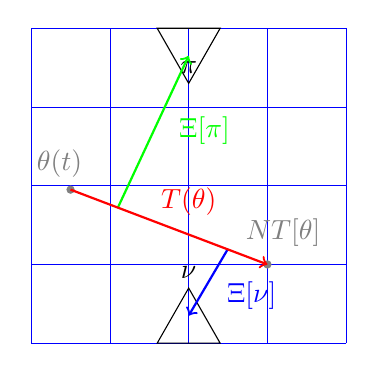
\begin{tikzpicture}
                \draw[step=1cm,blue,very thin] (-2,-2) grid (2,2);
                \draw (0.4, -2) node[anchor=north]{}
                -- (-0.4,-2) node[anchor=north]{}
                -- (0,-1.3) node[anchor=south]{$\nu$}
                -- cycle;
                \draw (0.4, 2) node[anchor=north]{}
                -- (-0.4, 2) node[anchor=north]{}
                -- (0,1.3) node[anchor=south]{$\pi$}
                -- cycle;

                \fill [color=gray] (-1.5, -0.05) circle (1.5pt);
                \draw[color=gray] (-1.64,0.28) node {$\theta(t)$};

                \draw[thick,->, green] (-0.9,-0.28) --(0.0,1.65);
                
                \draw[color=green] (0.2,0.7) node {$\Xi[\pi]$};
                
                \draw[thick,->, blue] (0.5,-0.8) --(0.0,-1.65);
                
                \draw[color=blue] (0.8,-1.4) node {$\Xi[\nu]$};
                
                \fill [color=gray] (1,-1) circle (1.5pt);
                \draw[color=gray] (1.2,-0.6) node {$NT[\theta]$};
                
                \draw[thick,->, red] (-1.5,-0.05) -- (1,-1);

                \draw[color=red] (0.0,-0.2) node {$T(\theta)$};

                
            \end{tikzpicture}            
    
            
        \end{itemize}
            
        We update the $mustGoBack$ value:
        
        \label{check}
        \[
        mustGoBack =
        \begin{cases}
            \text{True},& \text{if } \Upsilon \leq 90\degree \\
            \text{False}.& \text{otherwise}
        \end{cases}
        \]
        
        
        \textbf{Where:}
        
        \begin{itemize}
        
            \item $\Upsilon$ is the angle from $T(\theta)$ and $CD[\theta]$
            
            \item $CD[\theta]$ is the segment between $\theta$ and $\nu$
        
        \end{itemize}
        
        \textbf{\textit{For Example} $\Upsilon$ is:}
        
        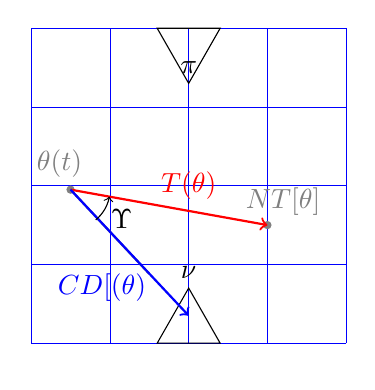
\begin{tikzpicture}
        
        \coordinate (origo) at (-1.5, -0.05); %A(t+1)
        \coordinate (pivot) at (0.0,-1.65);
        
            \draw[step=1cm,blue,very thin] (-2,-2) grid (2,2);
            \draw (0.4, -2) node[anchor=north]{}
            -- (-0.4,-2) node[anchor=north]{}
            -- (0,-1.3) node[anchor=south]{$\nu$}
            -- cycle;
            \draw (0.4, 2) node[anchor=north]{}
            -- (-0.4, 2) node[anchor=north]{}
            -- (0,1.3) node[anchor=south]{$\pi$}
            -- cycle;

            \fill [color=gray] (-1.5, -0.05) circle (1.5pt);
            \draw[color=gray] (-1.64,0.28) node {$\theta(t)$};

            
            \fill [color=gray] (1,-0.5) circle (1.5pt);
            \draw[color=gray] (1.2,-0.2) node {$NT[\theta]$};
            
            \draw[very thin] (origo) -- ++(-10.2:2.5) coordinate (bob);
            
            \draw[thick,->, red] (-1.5,-0.05) -- (1,-0.5);
            
            \draw[thick,gray] (origo) -- ++(1,-1.07) node (mary) [black,below] {};
            
            \draw[thick,->, blue] (-1.5,-0.05) -- (0.0,-1.65);
            
            
            \draw[color=red] (0,0) node {$T(\theta)$};

            \draw[color=blue] (-1.1,-1.3) node {$CD[(\theta)$};
            
            \pic [draw, ->, "$\Upsilon$", angle eccentricity=1.5] {angle = mary--origo--bob};
            
            
        \end{tikzpicture}
        
        \textbf{And:}
        
        \[
        \beta =
        \begin{cases}
            \text{$Check$ $NextIteration$ $mustGoBack$},& \text{if } mustGoBack = True \\
            \text{$Depot$},& \text{otherwise}
        \end{cases}
        \]
        
        \item If $|N(\theta)| \geq 1$
        
        \[
            \beta = 
            \begin{cases}
                None,& \text{if } \Phi = None \\
                \psi$ $ to$ $ \theta',& \text{otherwise if } \Phi = Pass \\
                Depot,& \text{otherwise if } \Phi = Depot \\
                Depot,& \text{otherwise if } \Phi = \{Pass, Depot\}\\
                None,& \text{otherwise}
            \end{cases}
        \]    
        
        \textbf{Where\footnote{Q-Learning purpose.}:}
        
        \begin{itemize}
        
            \item $\theta'$ $|$ $\theta' \in N(\theta) \wedge \forall\theta'' \in N(\theta)$, $v^{*}(\theta'$) = \textbf{max}$(v^{*}(\theta''))$

        \end{itemize}
        
        If $\Phi = \{Depot\}¨$ then:
        
        \[
            \rho = 
            \begin{cases}
                \nu,& \text{if }  Q(\nu) > Q(\pi) \\
                \pi,& \text{otherwise if } Q(\pi) > Q(\nu) \\
                \nu,& \text{otherwise if } \Xi[\nu] \leq \Xi[\pi] \\
                \pi,& \text{otherwise} \\
            \end{cases}
        \]    
            
        We update the usually mustGoBack value:
        
        \[
        mustGoBack =
        \begin{cases}
            \text{True},& \text{if } \Upsilon \leq 90\degree \\
            \text{False}.& \text{otherwise}
        \end{cases}
        \]
        
        \textbf{And:}
        
        \[
        \beta =
        \begin{cases}
            \text {$Check$ $NextIteration$ $mustGoBack$},& \text{if } mustGoBack = True \\
            \text{$Depot$},& \text{otherwise}
        \end{cases}
        \]
    
    \end{enumerate}
    
    \item In the $\epsilon$ case we have \textit{modified \textbf{MGEO} algorithm:}
    
    \begin{enumerate}
    
        \item If $N(\theta) = \emptyset$:
    
        \[
            \rho = 
            \begin{cases}
                \nu,& \text{if } \Xi[\nu] \leq \Xi[\pi] \\
                \pi,& \text{otherwise if } \Xi[\pi] > \Xi[\nu] \\
            \end{cases}
        \]
    
        
        We choose a $\rho$ and set:
        
        \[
            mustGoBack =
            \begin{cases}
                \text{True},& \text{if } \Upsilon \leq 90\degree \\
                \text{False}.& \text{otherwise}
            \end{cases}
        \]
        
        \textbf{And:}
        
        \[
        \beta =
        \begin{cases}
            \text {$Check$ $NextIteration$ $mustGoBack$},& \text{if } mustGoBack = True \\
            \text{$Depot$},& \text{otherwise}
        \end{cases}
        \]
        
        \item If $|N(\theta)| \geq 1$:
        
        $\forall\theta' \in N(\theta) \Rightarrow$
        
        \[
            \rho[\theta'] =
            \begin{cases}
                \nu,& \text{if } \textbf{dist}(NT[\theta'], \nu) \leq \textbf{dist}(NT[\theta'], \pi) \\
                \pi,& \text{otherwise}
            \end{cases}
        \]
        
        \textbf{Where:}
        
        \begin{itemize}
        
            \item $\rho[\theta']$ $\Rightarrow$ Nearest $\rho$ for $\theta'$
        
        \end{itemize}
        
        $\theta$ passes $\psi$ to $\vartheta$, where:
        \[
            \forall\theta' \in N(\theta), \exists\vartheta \in N(\theta) \textbf{ | }\textbf{dist}(NT[\vartheta], \rho[\vartheta]) = \textbf{min}(\textbf{dist}(NT[\theta'], \rho[\theta']))
        \]
        
        
        
    \end{enumerate}
    
    In this case we only update Q-Sets, NO EXPLOITATION
    
\end{itemize}
    
    Obviously we always update Q-Sets for any action that we do.
    
\subsection{Alpha/Gamma}

Important things are Q-Learning's parameters:

\[
    \alpha= 0.5
\]

\[
    \gamma= 0.2
\]

\textbf{Where:}

\begin{itemize}

    \item $\alpha$ is the learning-rate. If $\lambda$ function\footnote{\textbf{Remember:} It is the Reward Function.} or transition function is stochastic (random), then $\alpha$ should change over time. $\alpha$ should $\approx$ zero at $\infty$.

    \item $\gamma$ represents future $\lambda$. It can affect learning quite a bit. If $\gamma = 1$, the agent values future reward JUST AS MUCH as current reward. If an agent does something good this is JUST AS VALUABLE as doing this action directly. So learning doesn't work at that well at high $\gamma$ values.

    Conversely, $\gamma = 0$ will cause the agent to only value immediate rewards, which only works with very detailed $\lambda$ functions.

\end{itemize}

Sperimentally, for our scenarios, we want that $\alpha$ is balanced between the past and the future and we also want the value of $\gamma$ that it is small, because the scenario change frequently. So we need to do an high weight to the rewards that we will receive compared to the past learnings.  


\section{Conclusions: Performances in the Two Possible Scenarios}

We have tested two possible scenarios\footnote{To see differences with learning.}:

\begin{itemize}

    \item Repeated Routes $Rep$;
    
    \item Randomic Routes $Rnd$.
    
\end{itemize}

\begin{figure}[H]
    
    \subfloat{{\includegraphics[width=8.1cm,height=\textheight,keepaspectratio]{./Images/score_static.jpg} }}%
    \qquad
    \subfloat{{\includegraphics[width=8.1cm,height=\textheight,keepaspectratio]{./Images/score_random.png} }}%
    
    \caption{Plot Score $Rep$ vs $Rnd$}
    
    \label{fig:Score}%
\end{figure}

Figure \ref{fig:Score}: Score in $Rep$ is less than $Rnd$, but both of them have same convergence.

\begin{figure}[H]
    
    \subfloat{{\includegraphics[width=8.1cm,height=\textheight,keepaspectratio]{./Images/energy_move_routing_static.jpg} }}%
    \qquad
    \subfloat{{\includegraphics[width=8.1cm,height=\textheight,keepaspectratio]{./Images/energy_move_routing_random.png} }}%
    
    \caption{Plot Energy Consumed $Rep$ vs $Rnd$}
    
    \label{fig:Energy}%
\end{figure}

Figure \ref{fig:Energy}: In $Rep$ we exploit more the learning $\rightarrow$ So energy consumed is less, because it is avoided many times to go to $\pi$ or $\nu$.

\begin{figure}[H]
    
    \subfloat{{\includegraphics[width=8.1cm,height=\textheight,keepaspectratio]{./Images/ratio_delivery_detected_static.jpg} }}%
    \qquad
    \subfloat{{\includegraphics[width=8.1cm,height=\textheight,keepaspectratio]{./Images/ratio_delivery_detected_random.png} }}%
    
    \caption{Plot Ratio for Delivery Detected $Rep$ vs $Rnd$}
    
    
    \label{fig:Ratio}%
\end{figure}

\begin{figure}[H]
    
    \subfloat{{\includegraphics[width=8.1cm,height=\textheight,keepaspectratio]{./Images/number_of_events_to_depot_static.jpg} }}%
    \qquad
    \subfloat{{\includegraphics[width=8.1cm,height=\textheight,keepaspectratio]{./Images/number_of_events_to_depot_random.png} }}%
    
    \caption{Plot Number of Events to Depot $Rep$ vs $Rnd$}
    
    \label{fig:Number_Events}%
\end{figure}

Figure \ref{fig:Ratio} $\&$ Figure \ref{fig:Number_Events}::Ratio of Delivery and Number of Events to Depot is pratically the same in both scenarios and also for MGEO and AI\_Routing\footnote{\ref{fig:Number_Events} is the same of \ref{fig:Ratio}, because both of them are dependent values.}.


\begin{figure}[H]
    
    \subfloat{{\includegraphics[width=8.1cm,height=\textheight,keepaspectratio]{./Images/event_mean_delivery_time_static.jpg} }}%
    \qquad
    \subfloat{{\includegraphics[width=8.1cm,height=\textheight,keepaspectratio]{./Images/event_mean_delivery_time_random.png} }}%
    
    \caption{Plot Mean Delivery Time $Rep$ vs $Rnd$}
    
    \label{fig:Mean_Delivery}%
\end{figure}

Figure \ref{fig:Mean_Delivery}: \textbf{Important:} We deliver a lot of $\Gamma$ and for this reason the score isn't high, but Mean Time is a high $\rightarrow$ For each $\psi$ we have a wait 3 times higher than MGEO.

\begin{figure}[H]
    
    \subfloat{{\includegraphics[width=8.1cm,height=\textheight,keepaspectratio]{./Images/routing_time_mission_time_static.jpg} }}%
    \qquad
    \subfloat{{\includegraphics[width=8.1cm,height=\textheight,keepaspectratio]{./Images/routing_time_mission_time_random.png} }}%
    
    \caption{Plot $\frac{Routing Time}{Mission Time}$ $Rep$ vs $Rnd$}
    
    \label{fig:Final}%
\end{figure}

Figure \ref{fig:Final}: With few drones we have good results than MGEO. With more drones MGEO is in advantage.




\subsection{Conclusions}

MGEO Algorithm is better than us, also with 2 Depot's Scenario. Our approach is enough strong to deliver an high number of $\Gamma$, but it delivers each $\psi$ with high $\xi$, in average: This is the \textbf{Failure Point} $\rightarrow$ For a future work it's important work on this aspect.

On other hand, the proposed algorithm has consistently low battery consumption, as expected.

Luckly there aren't too many differencess between $Rep$ and $Rnd$. We have same good performance also in $Rnd$ $\rightarrow$ With our $\alpha$ and $\gamma$ parameters algorithm can adapt fastly to changing on the scenario ($Rnd$), without a large exploiting of past knowledges ($Rep$).
\section{Components' Contribute}

\begin{itemize}

    \item \textbf{Giordano:} With other components he decided what it is better to implement $\rightarrow$ It also briefly fix some code errors $\rightarrow$ Mainly he is the main responsible for the writing and the revision of the Report and for every formalism realized in it.
    
    
    \item \textbf{Mattia:} He worked on the design and implementation of the future development algorithms and at plotting.
    
    \item \textbf{Michele:} He took part in the design of the algorithm and its implementation, of both things he is the main author. He also collaborated in drafting the report, writing part of it, revising it and collaborating in writing the formulas.
    
\end{itemize}


\textbf{\textit{THANKS FOR YOUR ATTENTION :)}}



\end{document}
